\documentclass[12pt, twoside]{article}
\usepackage{amsmath, amssymb, amsthm}
\usepackage{bm, bbm}
\usepackage{algorithm}
\usepackage{algpseudocode}
\usepackage{float, graphicx, fullpage, parskip, subcaption, setspace, multicol}
\usepackage{comment}
\usepackage{url}
\usepackage{enumitem}
\usepackage{hyperref}
\usepackage{natbib}
\usepackage[usenames,dvipsnames]{xcolor}
\usepackage{nicematrix}
\usepackage{csquotes}
\usepackage{caption}

%
\captionsetup{belowskip=0pt}

% Define some colors
\definecolor{SkyBlue}{RGB}{14, 118, 188}
\definecolor{BrightRed}{RGB}{223, 82, 78}
\definecolor{Green638}{RGB}{165,255,118} % from colours.cafe on instagram; pallete638

% Set up colorful hyperlinks without any silly green boxes
\hypersetup{pdfborder = {0 0 0.5 [3 3]}, colorlinks = true, linkcolor = BrightRed, citecolor = SkyBlue}

\bibliographystyle{apalike}

% Math macros
\DeclareMathOperator*{\argmax}{arg\,max}
\DeclareMathOperator*{\argmin}{arg\,min}

\newcommand\numberthis{\addtocounter{equation}{1}\tag{\theequation}} % useful if we want to number one equation inside an align*
\newcommand\numbereqn{\addtocounter{equation}{1}\tag{\theequation}}

\newcommand{\R}{\mathbb{R}} % boldfaced R for the reals
\newcommand{\E}{\mathbb{E}} % boldfaced E for expectations
\def\P{\mathbb{P}} % boldfaced P for probability. overriding \P for paragraph symbol

\newcommand{\calP}{\mathcal{P}} % caligraphic P for a generic distribution
\newcommand{\calQ}{\mathcal{Q}} % caligraphic Q for another generic distribution
\newcommand{\calF}{\mathcal{F}} % caligraphic F, typically for sigma-algebras

\newcommand{\ind}[1]{\mathbbm{1}\left( #1 \right)} % indicator function, with an argument
\newcommand{\var}[1]{\textrm{Var}\left( #1 \right)} % variance
\newcommand{\cov}[2]{\textrm{Cov}\left( #1, #2 \right)} % covariance
\newcommand{\sign}[1]{\textrm{sign}\left(#1\right)} % sign
\newcommand{\parallelsum}{\mathbin{\|}} % for double bar to behave like a binary operation
\newcommand{\kl}[2]{\textrm{KL}\left(#1 \mid \parallelsum \# \right)} % KL divergence with two arguments


% distributions
\newcommand{\normaldist}[2]{\mathcal{N}\left(#1,~#2\right)} % normal distribution
\newcommand{\mvnormaldist}[3]{\mathcal{N}_{#1}\left(#2,~#3\right)} % multivariate normal distribution
\newcommand{\gammadist}[2]{\textrm{Gamma}\left(#1,~#2\right)} % gamma distribution
\newcommand{\igammadist}[2]{\textrm{Inv.~Gamma}\left(#1,~#2\right)} % inverse gamma
\newcommand{\binomialdist}[2]{\textrm{Binomial}\left(#1,~#2\right)} % Binomial
\newcommand{\berndist}[1]{\textrm{Bernoulli}\left(#1\right)} % Bernoulli
\newcommand{\poisdist}[1]{\textrm{Poisson}\left(#1\right)} % Poisson
\newcommand{\hafltdist}[2]{\textrm{half-t}_{\#1}\left(#2\right)} %half-t
\newcommand{\unifdist}[2]{\textrm{Uniform}\left(#1,~#2\right)} % uniform
\newcommand{\betadist}[2]{\textrm{Beta}\left(#1,~#2\right)} % Beta distribution

% bolded alphabet time
\newcommand{\by}{\bm{y}}
\newcommand{\bx}{\bm{x}}
\newcommand{\bz}{\bm{z}}
\newcommand{\bw}{\bm{w}}

% bolded capitalized alphabet
\newcommand{\bY}{\bm{Y}}
\newcommand{\bX}{\bm{X}}

% bolded greek alphabet time!
\newcommand{\btheta}{\boldsymbol{\theta}}
\newcommand{\bbeta}{\boldsymbol{\beta}}

%overline time
\newcommand{\ybar}{\overline{y}}
\newcommand{\xbar}{\overline{x}}
\newcommand{\mubar}{\overline{\mu}}

% for maximal laziness, anytime we need to refer to a generic prior, posterior, joint, or marginal density, we can use the follwing
\newcommand{\prior}{p(\theta)}
\newcommand{\like}{p(\by \vert \theta)}
\newcommand{\marg}{p(\by)}
\newcommand{\joint}{p(\by,\theta)}
\newcommand{\post}{p(\theta \vert \by)}

% Theorem-like declarations
\theoremstyle{plain}
\newtheorem{theorem}{Theorem}
\newtheorem{corollary}[theorem]{Corollary}
\newtheorem{lemma}[theorem]{Lemma}
\newtheorem{proposition}[theorem]{Proposition}

\theoremstyle{definition}
\newtheorem{definition}[theorem]{Definition}

\newtheorem{ex}{Example}
\newenvironment{example}{\begin{ex}}{ \hfill $\blacksquare$\end{ex}}


\theoremstyle{remark}
\newtheorem{remark}[theorem]{Remark}

% comment fields
\newcommand{\skd}[1]{\textcolor{red}{[skd]: #1}} % includes all of the macros and sets default layout and formating

\title{Your title here}
\author{Your names here}
\begin{document}
\onehalfspacing % don't change the spacing
\maketitle

\section{Introduction}
You should write an introduction.
The last paragraph of your introduction should provide an outline for the rest of the paper. 
C.f. most published papers whose introductions include a sentence like ``The rest of this paper is organized as follows'' or ``Here is a plan for the rest of the paper.''

\section{Body of the paper}

Depending on your specific choice of project, you should use as many sections as needed.
Look to the published literature for guidance on how to organize different sections. 
For empirical analyses, generally the second section introduces the data and provides some literature review. 
That is often followed by separate sections describing the models \& methods used, empirical results (on simulated and/or real data, as necessary), and a discussion.
For methodological and theoretical works, the structure is similar.

There is not one set standard and I encourage you to use whatever organization seems most effective to you. 

You should use figures and tables as appropriate. 
Figure~\ref{fig:bayes} is an example; it shows Rev. Thomas Bayes.

\begin{figure}[H] % H forces the figure to appear in this location, h! tries really hard to do the same thing
\centering
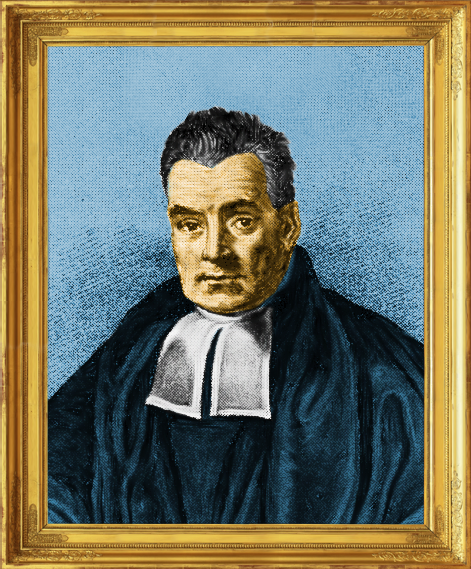
\includegraphics[width = 0.25\textwidth]{bayes} % no need to specify a file extension & pay attention to scaling by width!
\caption{All figures must have a caption \textit{below} the figure}
\label{fig:bayes} % useful for hyperref'ing later
\end{figure}

Sometimes you need to include multi-part figures like Figure~\ref{fig:multipart_figure}.
Figure~\ref{fig:bayes2} shows Rev. Thomas Bayes while Figures~\ref{fig:lindley} and~\ref{fig:box} show pictures of Dennis Lindley and George E.P. Box, respectively.
\begin{figure}[H]
\begin{subfigure}[b]{0.32\textwidth}
\centering
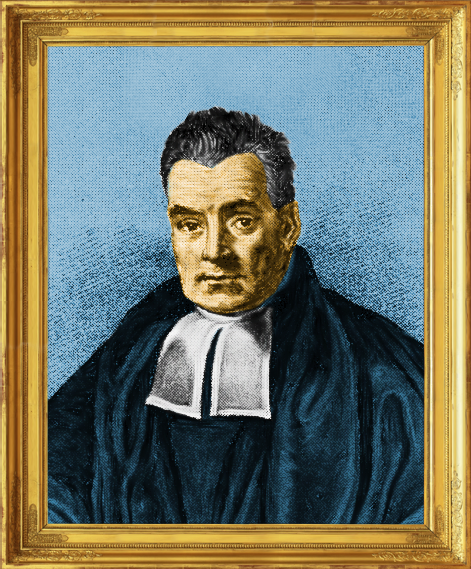
\includegraphics[width = \textwidth]{bayes}
\caption{}
\label{fig:bayes2}
\end{subfigure}
\begin{subfigure}[b]{0.32\textwidth}
\centering
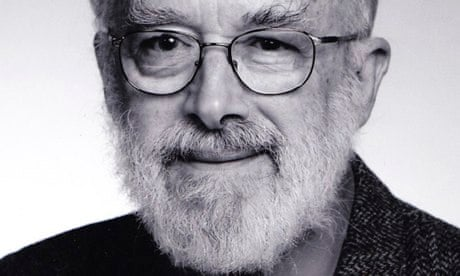
\includegraphics[width = \textwidth]{lindley}
\caption{}
\label{fig:lindley}
\end{subfigure}
\begin{subfigure}[b]{0.32\textwidth}
\centering
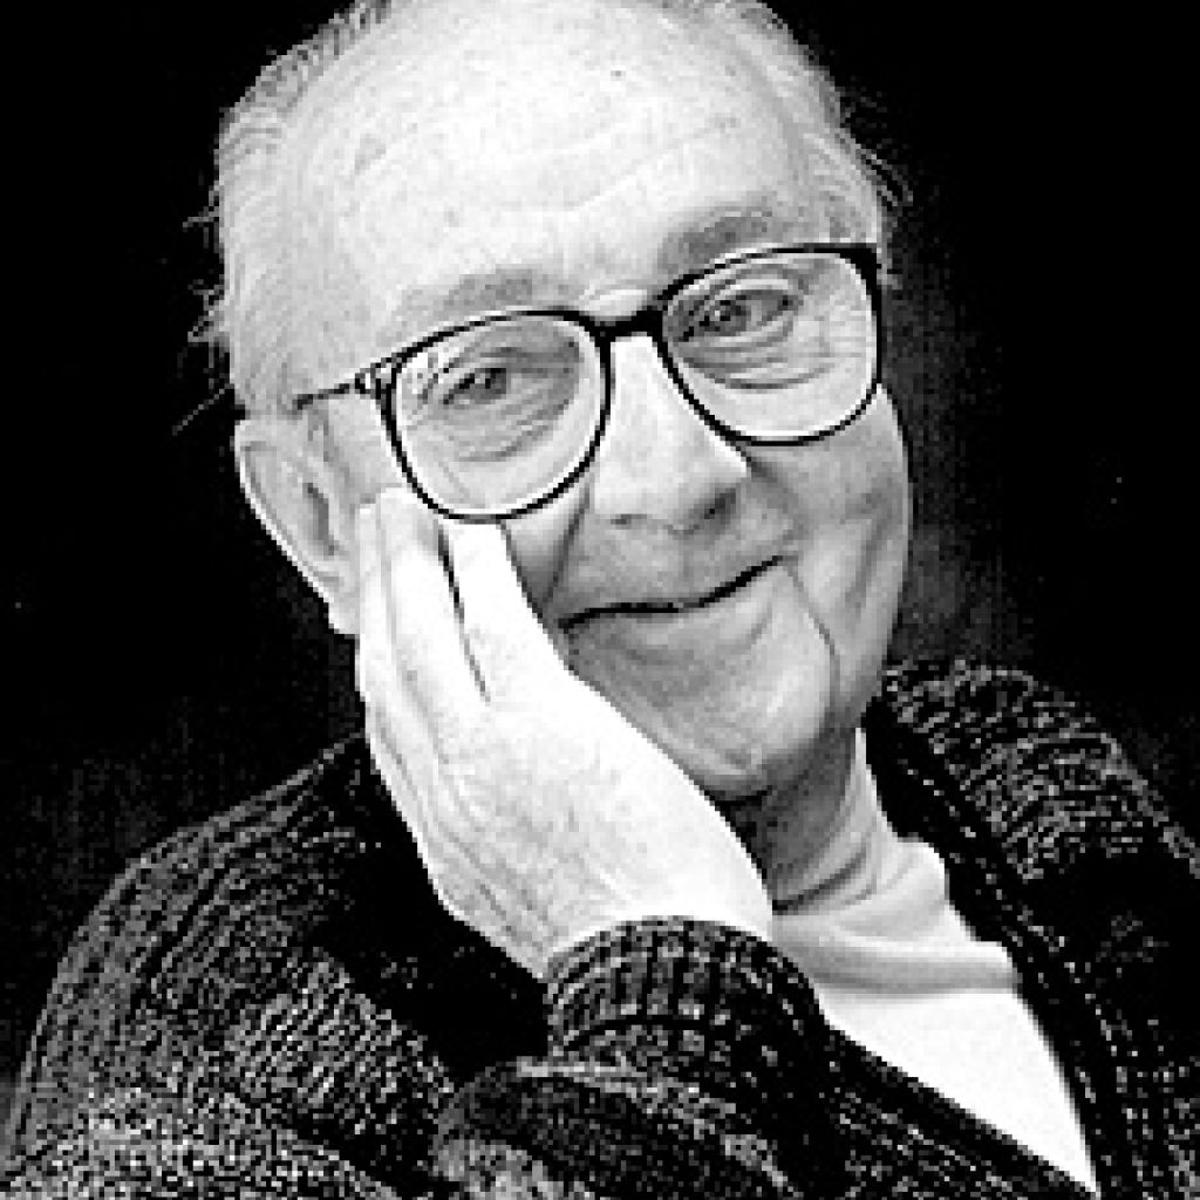
\includegraphics[width = \textwidth]{box}
\caption{}
\label{fig:box}
\end{subfigure}
\caption{Thomas Bayes (a), Dennis Lindley (b), and George E.P. Box (c)}
\label{fig:multipart_figure}
\end{figure}


You might find it necessary to include a Table to, e.g., report the results of a comprehensive simulation study.
Here is one such example

\begin{table}[H]
\centering
\caption{Table captions go above the table. Try to avoid unnecessary vertical lines between columns and horizontal lines between non-terminal rows}
\label{tab:results}
\begin{tabular}{lcr} % note the 
\hline
Column A & Column B & Column C \\ \hline
1 & 2 & 3 \\
4 & 5 & 6 \\ \hline
\end{tabular}
\end{table}

\section{Discussion}
You should conclude your report with a short discussion.
Immediately following the discussion should be a list of references.
If you do not already use BibTeX and natbib, now is a great time to learn!
You should cite any sources using the commands \texttt{citet} for inline references and \texttt{citep} for parenthetical references. 
So you would use \texttt{citet} to write something like ``\citet{Deshpande2019_mSSL} introduced an EM-like algorithm for simultaneous variable and covariance selection in multi-outcome linear models'' and you would use \texttt{citep} for a sentence like ``Spike-and-slab priors can be effectively deployed to perform simultaneous variable and covariance selection in multi-outcome linear models \citep{Deshpande2019_mSSL}.''

You should save your references in a \texttt{.bib} file that is located in the same directory as your LaTeX files.

\bibliography{references}

\end{document}
